% help.
\documentclass{beamer}
\usetheme{Boadilla}
\usepackage{graphicx}
\usepackage{textcomp}
\usepackage{amsmath}
\usepackage{mathtools}
\usepackage{tikz}
\usetikzlibrary{arrows,decorations.pathmorphing,backgrounds,positioning,fit,calc,shapes.geometric}
\usepackage{gensymb}
\usepackage{subcaption}
\usetikzlibrary{arrows,calc}
\tikzset{
%Define standard arrow tip
>=stealth',
%Define style for different line styles
help lines/.style={dashed, thick},
blue block/.style={fill=blue!20,draw=blue!50},
axis/.style={<->},
important line/.style={thick},
connection/.style={thick, dotted},
}
\setlength{\abovedisplayskip}{0pt}
\setlength{\belowdisplayskip}{0pt}
\setlength{\abovedisplayshortskip}{0pt}
\setlength{\belowdisplayshortskip}{0pt}

\title{NEXMD with Sander's QM/MM}
\subtitle{NonAdiabatic Dynamics Using AMBER}
\author{Dustin Tracy}
\institute{University of Florida}
\date{06/30/20}

\begin{document}
% Title
\begin{frame}
  \titlepage
\end{frame}

\section{background}
\begin{frame}
  \frametitle{Conjugate Organic Molecules}
\begin{columns}[c]
  \column{0.45\textwidth}
  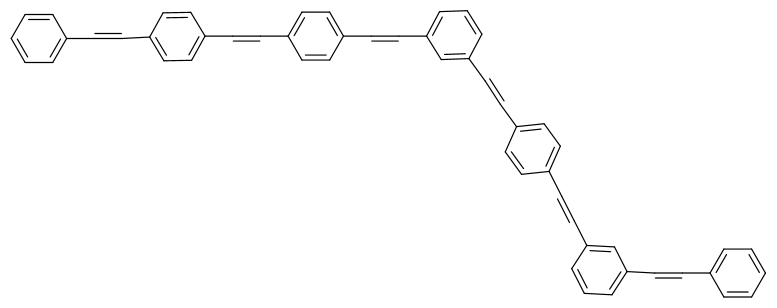
\includegraphics[width=\textwidth]{Images/com}
  \column{0.45\textwidth}
  \begin{itemize}
    \item They tend to be very good at energy transfer
    \item 2 $\rightarrow$ 3 $\rightarrow$ 4
    \item Excited state dynamics can speed or slow this transition.
  \end{itemize}
\end{columns}
\begin{block}{Question}
  How can we simulate this?
\end{block}
\end{frame}

\begin{frame}
  \frametitle{Possible Solutions}
\begin{itemize}
  \item Run Classical Ground State Dynamics then perform Excited Sated Energy Calculations on snapshots
  \begin{itemize}
    \item Excited State dynamics could be different.
    \item In the molecules I studied for example, the excited state had a
      much more planer dynamics than ground state
  \end{itemize}
  \item Run dynamics using the average forces of all the relevant excited states (Ehrenfest)
  \begin{itemize}
    \item Often the average force is not a very good approximation of either. 
  \end{itemize}
  \item Run a swarm of trajectories that are allowed to switch between different
    states (FSSH)
  \begin{itemize}
    \item The proportion of the population that are on a certain state represent the probability of the state.
    \item Can be very computationally expensive
  \end{itemize}
\end{itemize}
\end{frame}

\section{Fewest Switches Surface Hopping}
\begin{frame}
  \frametitle{General Outline of Dynamics}
  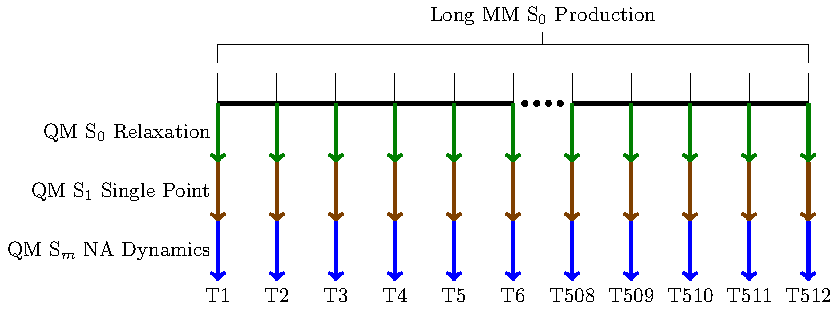
\includegraphics[width=0.7\textwidth]{Images/simulations}
\begin{block}{Example Times}
\begin{itemize}
    \item Perform a long MM trajectory
    \item Take snapshot every 1 PS, run QM Ground State for relaxation
    \item Excite the System
    \item Allow each of these trajectories relax independently
    \begin{itemize}
      \item Sum the population in each state to get state probabilities over time
      \item Analyze absorption and emission properties by looking at frequencies and oscillator strengths
    \end{itemize}
\end{itemize}

\end{block}
\end{frame}

\begin{frame}
  \frametitle{Long MM Trajectory}
\begin{block}{Sampling}
    The goal of our analysis is to derive the probability of states of a solute in solution.
    Their are of possible conformations for a molecule. If you
    then include a solvent, the number of snapshots needed to accurately sample
    the phase space increased even more. A long run is necessary for decent sampling.
\end{block}
\begin{block}{Guidelines}
 \begin{itemize}
  \item 1 ps time spacing between MM snapshots at 300K
  \item 500 samples for ~50 atoms in vacuum
 \end{itemize}
\end{block}
\end{frame}

\begin{frame}
  \frametitle{Ground State Calculations}
\begin{columns}[c]
  \column{0.45\textwidth}
\begin{figure}
  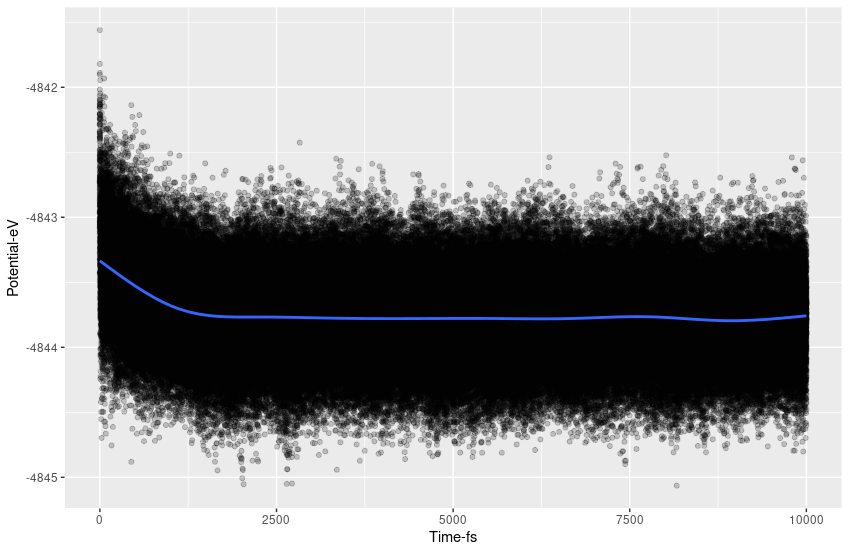
\includegraphics[width=\textwidth]{Images/qmgroundrelaxation}
  \caption{QM S$_0$ relaxation of PPV3-NO$_2$ in methanol.}
\end{figure}
 
  \column{0.45\textwidth}
  \begin{block}{}
    \begin{itemize}
      \item The Algorithm used to decide whether to jump is very sensitive to energies.
      \item QM/MM energies are not going to be the same as MM
      \item Some time is needed to properly relax
    \end{itemize}
  \end{block}
\end{columns}
\end{frame}

\begin{frame}
  \frametitle{Excite The System}
\begin{columns}[c]
  \column{0.45\textwidth}
  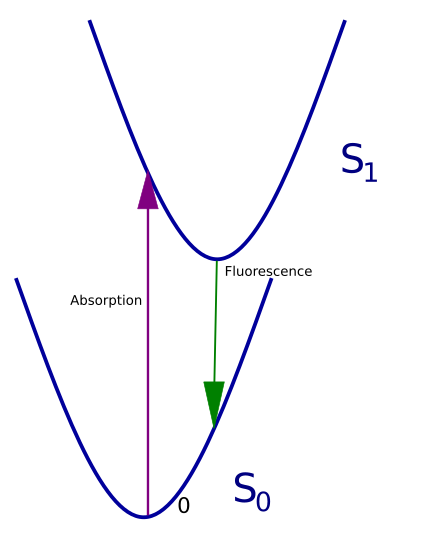
\includegraphics[width=\textwidth]{Images/abs_chart_mirror}
  \column{0.45\textwidth}
  \begin{block}{}
    \begin{itemize}
    \item We use laser excitations with a wave shape similar to that done in experiment
    \item Due to quantum uncertainty these states are also chosen based on the Franck-Condon principle
    \item Energy is not conserved (We're shooting a laser at it.)
    \item Velocities and Coordinates are maintained in this step
    \end{itemize}
  \end{block}
\end{columns}
\end{frame}

\begin{frame}
  \frametitle{Let the System Relax}
\begin{columns}[c]
  \column{0.45\textwidth}
  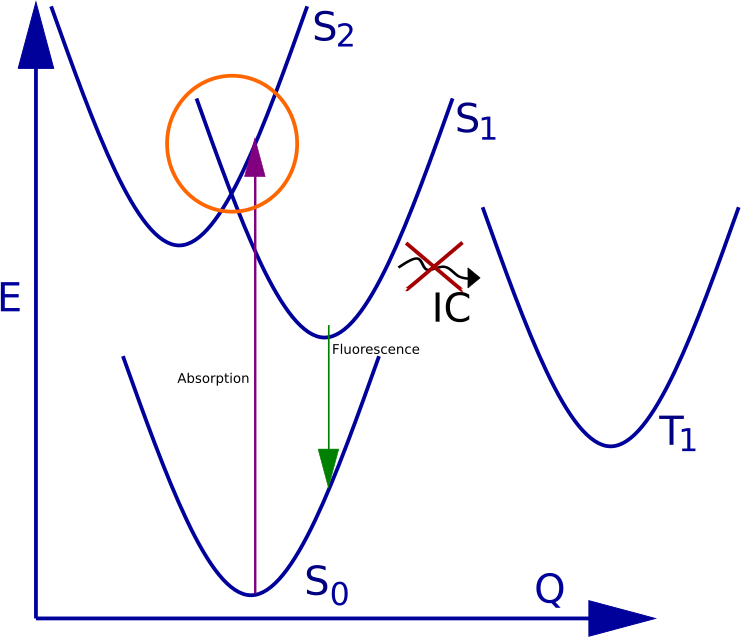
\includegraphics[width=\textwidth]{Images/abs_chart_modified}
  \column{0.45\textwidth}
  \begin{block}{}
    \begin{itemize}
    \item The molecule will start at a very high excited state
    \item When near a crossing of the energies, we have a very strong coupling, the state can shift
    \item When there's a switch the velocities of the atoms are adjusted to conserve energy
    \item Phosphorescence is not allowed
    \end{itemize}
  \end{block}
\end{columns}
\end{frame}

\begin{frame}
  \frametitle{Analyze The Results}
 \begin{columns}[c]
   \column{0.45\textwidth}
\begin{block}{Population Decay}
We can plot the proportion of trajectories in each states as a proxy to quantum
probabilities of the states. This provides a detailed view of state decay rates. 
\end{block}
\begin{block}{Excited State Energy Relaxation}
The molecule is suddenly placed outside of equilibrium. Modeling the excited
state relaxation provides some insight into how this energy is dissipated to the
thermostat, solvent, both.
\end{block}
   \column{0.45\textwidth}
\begin{block}{Evolution of the Electronic Wave Function}
The transition density matrix, needed for the calculation of the hopping
probabilities can be repurposed to follow the physical movement of the excited electron density during decay.
\end{block}
\begin{block}{Change in Vibrational Modes}
  Certain vibrational mode will be heavily coupled to adiabatic state
  transitions. Some of these could be very fast (Bonds) and others slower (Torsional).
\end{block}

 \end{columns} 
\end{frame}

\begin{frame}
  \frametitle{Why add QM/MM?}
  NEXMD can perform the above calculations already
\begin{block}{However}
  \begin{itemize}
    \item The choice to switch states is sensitive to energies
    \item (Solvatochromic) Shifts in emission and absorption energies are known to
    occur in solvents.
    \item Applications such as sensors, fluorescent tags, L.E.D's, etc, will include solvent.
    \item NEXMD uses SQM as a backend, which is part of AMBERTOOLS.
    \begin{itemize}
      \item This should make NEXMD trivial to use a library in AMBER
      \item Unfortunately it didn't.
    \end{itemize}
  \end{itemize}
\end{block}
\end{frame}

\begin{frame}
  \frametitle{How We Did It}
  \begin{center}
  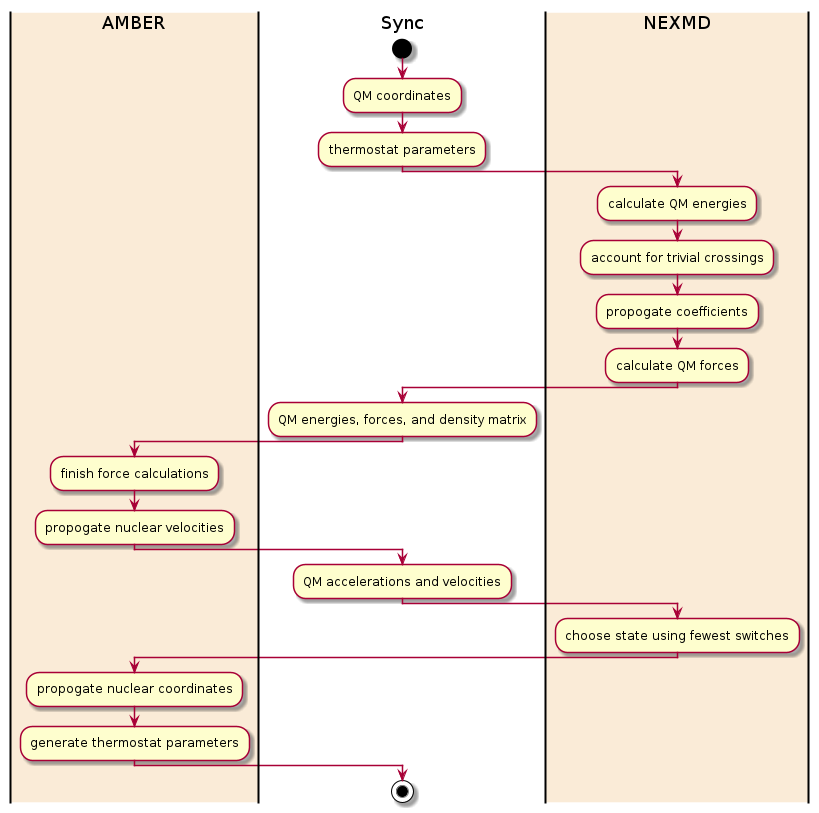
\includegraphics[width=0.6\textwidth]{Images/nasqm_overview.png}
  \end{center}
\end{frame}

\begin{frame}
  \frametitle{The Test Systems}
  \framesubtitle{polyphenylene vinylene oligimors}
\begin{columns}[b]
  \column{0.45\textwidth}
 \begin{figure}
  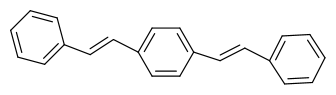
\includegraphics[width=\textwidth]{Images/ppv3.png}
  \caption{PPV3}
 \end{figure}
 
  \column{0.45\textwidth}
 \begin{figure}
  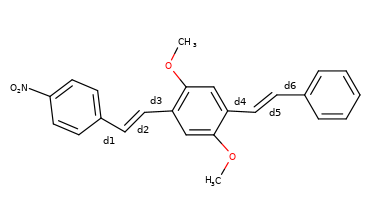
\includegraphics[width=\textwidth]{Images/ppvno2.png}
  \caption{PPV3-NO$_2$}
 \end{figure}
\end{columns}
\begin{block}{}
  \begin{itemize}
    \item These systems are smallish
    \item These systems are well studied
    \item The Hamiltonian is known to provide reasonable results
  \end{itemize}
\end{block}

\end{frame}



\end{document}
